\documentclass[tikz]{standalone}
% \input{styles_ondes.tex}
\usepackage[utf8x]{inputenc}
\usetikzlibrary{calc,arrows,fadings,decorations.pathreplacing,decorations.markings,patterns,shapes.geometric}
\tikzset{force/.style={->,ultra thick,rounded corners=4pt,color=blue,smooth,line cap=round}}


\begin{document}
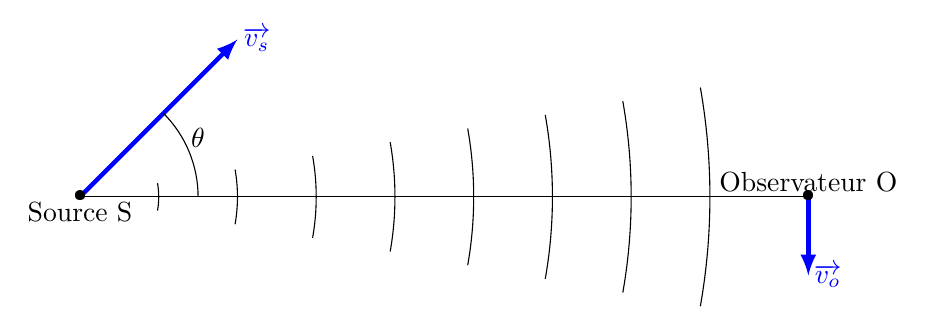
\begin{tikzpicture}[scale=1,inner sep=0pt, outer sep=2pt,>=latex]
\draw[force](0,0)--(2,2)node[right]{$\overrightarrow{v_s}$};
\draw[] (1.5,0) arc (0:45:1.5);
\node[] (ang) at (1.5,.75) {$\theta$};
\draw[force](9.25,0)--++(0,-1)node[right]{$\overrightarrow{v_o}$};
\draw(0,0)node{•}node[below]{Source S}--(9.25,0)node{•}node[above]{Observateur O};
\foreach \x in {1,2,3,4,5,6,7,8}{\draw (-10:\x) arc(-10:10:\x);}
\end{tikzpicture}
\end{document}